\chapter{High-Level Architecture}
% high level architecture
% how accomplish objectives from above
% what changes, rationale
% how it actually works
% checksums/persistence/how model is updated
% dealing with parallel edits
% updating clients
% presence awareness
% 1) architecture  (why) [distributed/reliable/multiple boards]
% 2) "new htink" - why
% design decisions
% new archi
% experience with it

\todo{Need a diagram to show how stuff connects}

In order to meet the objectives that we set in the new version of Calico, we decided that the architecture needed to be completely redesigned in order to support all the changes. The new architecture that we chose had to be able to support all the features, as well as easily support multiple users simultaneously. It also had to be accessible from anywhere, and had to be stable to prevent constant headaches when recoverying from crashes.

%\begin{figure}[h]
%\centering
%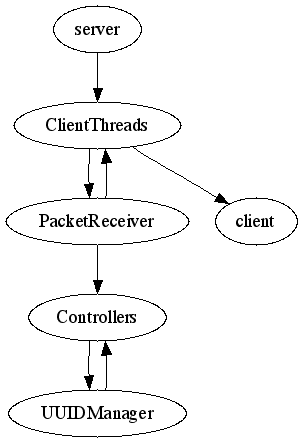
\includegraphics[width=0.8\textwidth]{calico_arch.png}
%\caption{Overview of Calico's Architecture}
%\label{fig:calico_arch}
%\end{figure}

The first change made was a switch from the original peer-to-peer system to a completely new client-server architecture. We believed that by using the client-server architecture, we could provide a centrally accessible service that would easily support multiple clients and still maintain stability. The server could act as a headless service that could be very powerful since it did not have to perform any client functions. This meant that the server could be dedicated to the task of managing all the interactions between clients, and could be much more stable than in a peer-to-peer context.

% Major change - java objects no longer used
One of the significant changes from the original Calico was the change in network communication design. The previous version of Calico had networking that was designed as a plugin, and was not fully integrated into the system. In this old design, when a change was made by another client, the entire change was saved to a Java object. This object was then serialized and sent in full over the network. The receiving client would deserialize this data, and then perform the change on its local drawing canvas. This process was very easy to implement, but had the cost of enormous overhead due to the constant serialization/deserialization process that would take place for each action. It also incurred the overhead of Java serialization, which would add much more data to the final packet then would ever be needed. All this overhead would quickly become apparent to users when the system would lag in response to many actions done in quick succession. Our goal was to streamline this process as much as possible so that we could reduce lag when the system was being heavily utilized.

To improve the responsiveness of Calico, and reduce the network overhead, I created a custom packet design that could be used by Calico to notify both the client and server when various actions were performed. These special packets provided exactly what was needed to effectively communicate changes to clients, and were reduced to the minimum size. Packets were byte arrays that were written directly to the wire, and based on various settings, they could be decoded back into their specific components. 



\begin{figure}[h!]
\centering

\begin{bytefield}{128}
  \bitbox{32}{packet size} & \wordbox{32}{command ID} & \bitbox{64}{command-specific data}
\end{bytefield}

\caption{Calico Packet}
\label{fig:calico_packet}
\end{figure}

This packet design was loosely based on the packet design of the Half-Life game engine \cite{todo}.As seen in the figure above, the packet was broken up into three main parts. The first four bytes of the packet was the length of the packet. This would tell the network system how much farther it needed to read to ensure it received the entire packet. The next four bytes held the command identifier. This number was used to tell the network system what this packet was about. Both the client and the server had a list of commands and their IDs, which was used to translate from a programmer-friendly command name to the command ID number. The remaining bytes could vary based on the specific command that was given. Each command had different parameters, which both the client and server were aware of, and could read the packet. By writing data directly to the wire, there was no overhead at all with inflated packet sizes -- each packet was as small as it could be. This made the network communication between the client and server incredibly efficient, and helped to reduce the lag, even when put under heavy usage.


%\section{Major Changes}
% move away from java objects being sent over the wire
% describe packet system

%\section{Maintaining Consistency}
% How data is sent back and forth between server and client
% How data is written to the controllers
% how parallel edits are dealt with
% 

%\section{Server Architecture}


%\section{Client Architecture}

% Components
% - Server
% - Client